\chapter{基于混合对数正太模型SAR图像目标检测}
\label{cha:china}

\section{引言}
\label{sec:chap2:sec1}
在使用恒虚警率的SAR图像目标检测方法中,对海杂波的精准建模是其中至关重要的问题。目前可以有效
对海杂波建模的分布模型有锐利分布,K分布,威布尔分布,对数高斯分布等。在本章中我采用混合对数正太
模型对强度SAR图像中的海杂波进行建模,实质上对数混合正太模型(lognormal mixture model)等价于强度SAR图像在对数域上的混合
高斯模型,因此可以采用EM方法估计分布参数,得到海杂波概率密度分布后应用牛顿迭代法计算分割阈值输出
检测的结果图像


\section{对数混合正太模型}
\label{sec:chap2:sec2}
  定义强度SAR图像中的像素值$\bf{x}$为一随机变量,当其满足式\ref{equ:chap2:LMM}中的分布时,我们称随机变量$\bf{x}$
  服从包含K个成分的混合对数正太分布。

    \begin{equation}
      \label{equ:chap2:LMM}
      {f_x}(x) = \mathop \Sigma \limits_{i = 1}^K {\alpha _i} \cdot \frac{1}{{\sqrt {2\pi } {\sigma _i}x}}\exp ( - \frac{{{{(\ln x - {\mu _i})}^2}}}{{2{\sigma ^2}}}),x > 0
    \end{equation}
  在式\ref{equ:chap2:LMM}中,$\alpha_i$, $\mu_i$, $\sigma_i(i=1,2,...,K)$为混合对数正太分布参数
  其中$\alpha_i$权重系数满足式\ref{equ:chap2:weigth}所示关系。混合对数正太分布为K个对数正太分布
  加权求和。$\mu_i$,$\sigma_i$为各独立的对数正太分布参数。

    \begin{equation}
      \label{equ:chap2:weigth}
      \sum\limits_{i = 1}^K {{\alpha _i} = 1,{\alpha _i} \ge 0} 
    \end{equation}

  对随机变量$\bf{x}$做形式变换,另$Y=\bf{x}$,我们可以推导出对于随机变量$Y$,其满足的概率密度函数如式\ref{equ:chap2:GMM}所示,显然
  随机变量$Y$满足含有K个分量的混合高斯分布,等价来讲对于强度SAR图像采用混合对数正太模型对海杂波进行建模
  等价于在SAR图像对数强度域上应用混合高斯模型,因此在该建模方法中,首先对强度SAR图像取对数变换到对数域,然后应用混合高斯
  模型描述海杂波的分布。

    \begin{equation}
      \label{equ:chap2:GMM}
        {f_Y}(y) = \mathop \Sigma \limits_{i = 1}^K {\alpha _i} \cdot \frac{1}{{\sqrt {2\pi } {\sigma _i}}}\exp ( - \frac{{{{(y - {\mu _i})}^2}}}{{2{\sigma ^2}}})
    \end{equation}


  \section{海杂波分布参数估计}

      在\ref{sec:chap2:sec2}节表明,混合对数正太分布在强度域与混合高斯分布在对数域上等价,因此混合正太
      分布中的参数计算可以采用目前现有的混合高斯模型参数计算方法。在文献[4]中表明了对于混合高斯模型,最大期望算法
      是一种高效的估计混合高斯分布参数的方法。因此在参数估计中,应用EM算法计算海杂波分布参数。参数迭代更新如式\ref{equ:chap2:paramupdate}
      所示。在该式中$\phi (y|{\mu _k},{\sigma _k})$为均值为$\mu_k$,标准差为$\sigma_k$的高斯分布,$n$为参与估计的杂波像素数量,
      $y$为取对数后的图像强度值。      

    \begin{equation}
      \label{equ:chap2:paramupdate}
      \begin{array}{*{20}{c}}
        {{\mu _k}^{i + 1} = \frac{{\sum\limits_{j = 1}^n {{\gamma _{jk}}{y_j}} }}{{\sum\limits_j^n {{\gamma _{jk}}} }}}\\
        {{\sigma _k}^{{\rm{i}} + 1} = \sqrt {\frac{{\sum\limits_{j = 1}^n {{\gamma _{jk}}({y_j} - {\mu _k}^{i + 1})} }}{{\sum\limits_j^n {{\gamma _{jk}}} }}} }\\
        {{\alpha _k}^{i + 1} = \frac{{\sum\limits_j^n {{\gamma _{jk}}} }}{n}}\\
        {{\gamma _{jk}} = \frac{{{\alpha _k}^i\phi ({y_j}|u_k^i,\sigma _k^i)}}{{\sum\limits_{k = 1}^K {{\alpha _k}^i\phi ({y_j}|u_k^i,\sigma _k^i)} }}}
      \end{array}
    \end{equation}

    受自然条件风速、风向的影响,同一SAR图像不同区域的杂波分布不尽相同,因此采用图\ref{fig:chap2:slide}所示的
    滑动窗进行局部杂波像素的选取,该滑动窗分为三个区域分别为检测像素区域,保护区域,杂波区域。合适大小的保护区域可以减少
    舰船目标像素对杂波统计分布参数估计的干扰。选定杂波像素值后,将其代入到式\ref{equ:chap2:paramupdate}中进行
    海杂波分布参数的迭代估计。

    \begin{figure}[H] % use float package if you want it here
      \centering
      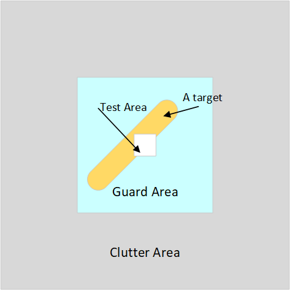
\includegraphics[width=0.5\textwidth]{slide.png}
      \caption{采用滑动窗进行自适应杂波参数估计,阴影所示像素用于杂波估计}
      \label{fig:chap2:slide}
    \end{figure}   
\section{应用LMM模型进行CFAR舰船检测}

\subsection{绘图}
\label{sec:draw}


本模板不再预先装载任何绘图包(如 \pkg{pstricks,pgf} 等),完全由用户来决定。
个人觉得 \pkg{pgf} 不错,不依赖于 Postscript。此外还有很多针对 \LaTeX{} 的
 GUI 作图工具,如 XFig(jFig), WinFig, Tpx, Ipe, Dia, Inkscape, LaTeXPiX,
jPicEdt, jaxdraw 等等。

\subsection{插图}
\label{sec:graphs}

强烈推荐《\LaTeXe\ 插图指南》!关于子图形的使用细节请参看 \pkg{subcaption} 宏包的说明文档。

\subsubsection{一个图形}
\label{sec:onefig}
一般图形都是处在浮动环境中。之所以称为浮动是指最终排版效果图形的位置不一定与源文
件中的位置对应\footnote{This is not a bug, but a feature of \LaTeX!},这也是刚使
用 \LaTeX{} 同学可能遇到的问题。如果要强制固定浮动图形的位置,请使用 \pkg{float} 宏包,
它提供了 \texttt{[H]} 参数,比如图~\ref{fig:xfig1}。


大学之道,在明明德,在亲民,在止于至善。知止而后有定;定而后能静;静而后能安;安
而后能虑;虑而后能得。物有本末,事有终始。知所先后,则近道矣。古之欲明明德于天
下者,先治其国;欲治其国者,先齐其家;欲齐其家者,先修其身;欲修其身者,先正其心;
欲正其心者,先诚其意;欲诚其意者,先致其知;致知在格物。物格而后知至;知至而后
意诚;意诚而后心正;心正而后身 修;身修而后家齐;家齐而后国治;国治而后天下
平。自天子以至于庶人,壹是皆以修身为本。其本乱而未治者 否矣。其所厚者薄,而其所
薄者厚,未之有也!

\hfill —— 《大学》


\subsubsection{多个图形}
\label{sec:multifig}

如果多个图形相互独立,并不共用一个图形计数器,那么
用 \texttt{minipage} 或者\texttt{parbox} 就可以。否则,请参看
图~\ref{fig:big1-subcaptionbox},它包含两个小图,分别是图~\ref{fig:subfig1}和
图~\ref{fig:subfig2}。推荐使用 \cs{subcaptionbox},因为可以像
图~\ref{fig:big1-subcaptionbox} 那样对齐子图的标题,也可以使用 \pkg{subcaption}
宏包的 \cs{subcaption}(放在 minipage中,用法同\cs{caption})或
是 \pkg{subfigure} 、\pkg{subtable}环境,像图~\ref{fig:big1-subfigure},不要再
用 \cs{subfloat}、\cs{subfigure} 和 \cs{subtable}。

\begin{figure}[h]
  \centering%
  \subcaptionbox{第一个小图形\label{fig:subfig1}}[3cm] %标题的长度,超过则会换行,如下一个小图。
    {
\includegraphics[height=3cm]{thu-fig-logo.pdf}}%
  \hspace{4em}%
  \subcaptionbox{第二个小图形,注意这个图略矮些。如果标题很长的话,它会自动换行\label{fig:subfig2}}
      {
\includegraphics[height=2cm]{thu-text-logo.pdf}}
  \caption{包含子图形的大图形(subcaptionbox示例)}
  \label{fig:big1-subcaptionbox}
\end{figure}
\begin{figure}[h]
  \centering%
  \begin{subfigure}{3cm}
    
\includegraphics[height=3cm]{thu-fig-logo.pdf}
    \caption{第一个小图形}
  \end{subfigure}%
  \hspace{4em}%
  \begin{subfigure}{0.5\textwidth}
    
\includegraphics[height=2cm]{thu-text-logo.pdf}
    \caption{第二个小图形,注意这个图略矮些。subfigure中同一行的子图在顶端对齐。}
  \end{subfigure}
  \caption{包含子图形的大图形(subfigure示例)}
  \label{fig:big1-subfigure}
\end{figure}

古之学者必有师。师者,所以传道受业解惑也。人非生而知之者,孰能无惑?惑而不从师,
其为惑也,终不解矣。生乎吾前,其闻道也固先乎吾,吾从而师之;生乎吾後,其闻道也亦
先乎吾,吾从而师之。吾师道也,夫庸知其年之先後生於吾乎!是故无贵无贱无长无少,道
之所存,师之所存也。

嗟乎!师道之不传也久矣,欲人之无惑也难矣。古之圣人,其出人也远矣,犹且从师而问焉;
今之众人,其下圣人也亦远矣,而耻学於师。是故圣益圣,愚益愚。圣人之所以为圣,愚
人之所以为愚,其皆出於此乎?爱其子,择师而教之,於其身也,则耻师焉,惑焉。彼童子
之师,授之书而习其句读者,非吾所谓传其道、解其惑者也。句读之不知,惑之不解,或师
焉,或不焉,小学而大遗,吾未见其明也。巫医、乐师、百工之人不耻相师,  士大夫之族
曰“师”曰“弟子”之云者,则群聚而笑之。问之,则曰:彼与彼年相若也,道相似也,位
卑则足羞,官盛则近谀。呜呼!师道之不复,可知矣。巫医、乐师、百工之人。吾子不齿,
今其智乃反不能及,其可怪也欤!圣人无常师。孔子师郯子、苌子、师襄、老聃。郯子之徒,
其贤不及孔子。孔子曰:“三人行,必有我师。”是故弟子不必不如师,师不必贤於弟子。
闻道有先後,术业有专攻,如是而已。

如果要把编号的两个图形并排,那么小页就非常有用了:
\begin{figure}
\begin{minipage}{0.48\textwidth}
  \centering
  
\includegraphics[height=2cm]{thu-whole-logo.pdf}
  \caption{并排第一个图}
  \label{fig:parallel1}
\end{minipage}\hfill
\begin{minipage}{0.48\textwidth}
  \centering
  
\includegraphics[height=2cm]{thu-whole-logo.pdf}
  \caption{并排第二个图}
  \label{fig:parallel2}
\end{minipage}
\end{figure}

李氏子蟠,年十七,好古文、六艺,经传皆通习之,不拘於时,学於余。余嘉其能行古
道,作师说以贻之。

\hfill —— 韩愈(唐)
